\section{Testing}
\begin{figure}
    \centering
    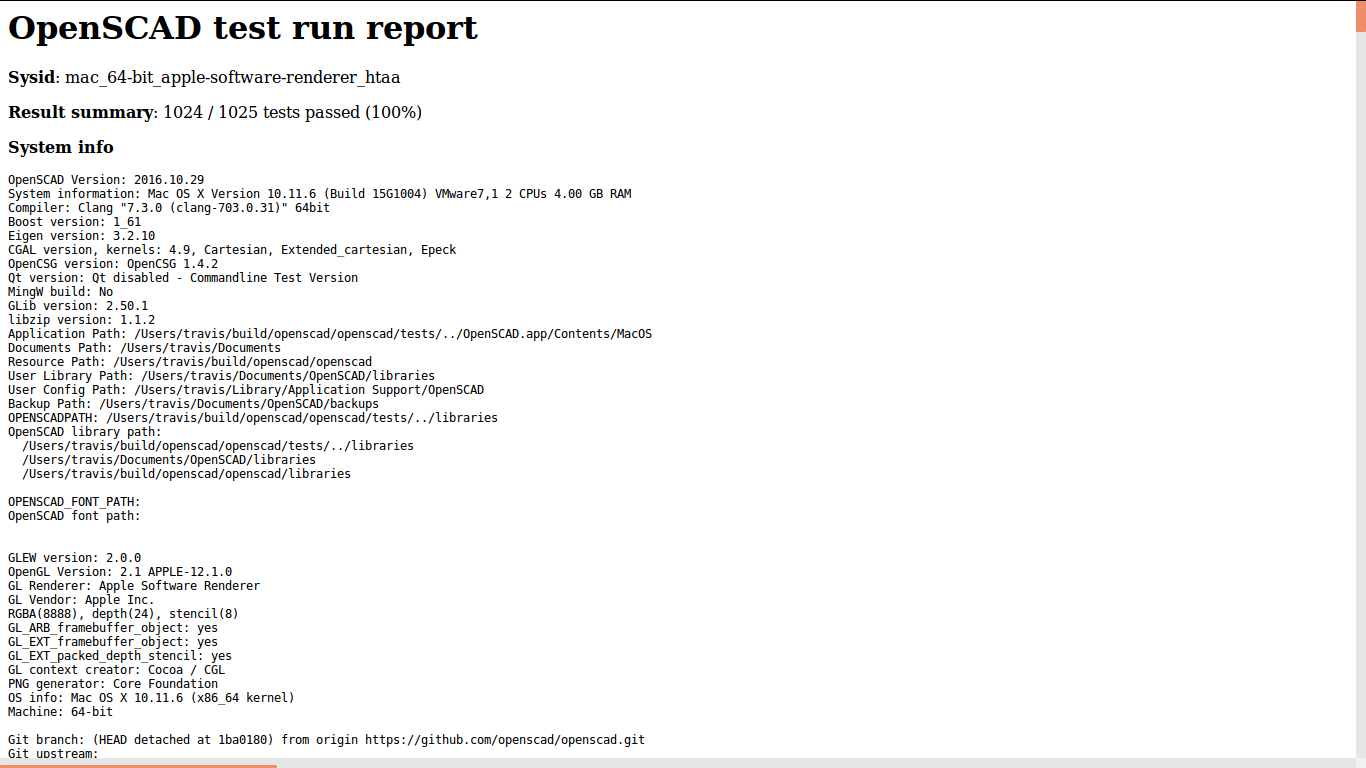
\includegraphics[width=\linewidth]{images/travisTestReport}
    \caption{Test Report by travis}
    \label{fig:travisTestReport}
\end{figure}

OpenSCAD is the software used by many of people all over the world and many web services as backend. so, it has to be perfect, Robust, reliable and bug-free. So, A very strong test suite is developed for testing this software and any component or feature that is to be integrated into OpenSCAD. And our project was able to pass all the task before getting Integrated into OpenSCAD.

Test Suit for OpenSCAD is developed using following two software:

\begin{enumerate}
    \item \textbf{cTest:} CTest is a testing tool distributed as a part of CMake. It can be used to automate updating (using CVS for example), configuring, building, testing, performing memory checking, performing coverage, and submitting results to a CDash or Dart dashboard system.
    cTest is used by OpenSCAD for testing the OpenSCAD on the local system of developers and it performs black box and regression testing of the software.
   
    \item \textbf{Travis CI:} Travis CI is a hosted, distributed continuous integration service used to build and test software projects hosted on GitHub.Open source projects may be tested at no charge via travis-ci.org. Private projects may be tested at the same location on a fee basis.
    Travis CI is used mainly for Installation testing on different OS and It also perform  black box and regression testing on different operating systems.
   
\end{enumerate}

Test Suit developed for OpenSCAD perform following type of testing:
 
 \begin{enumerate}
     \item \textbf{Installation Testing:} It is done by building the OpenSCAD from scratch on totally fresh installation of different operating systems. \ref{fig:travis}
   
     \begin{figure}
         \centering
         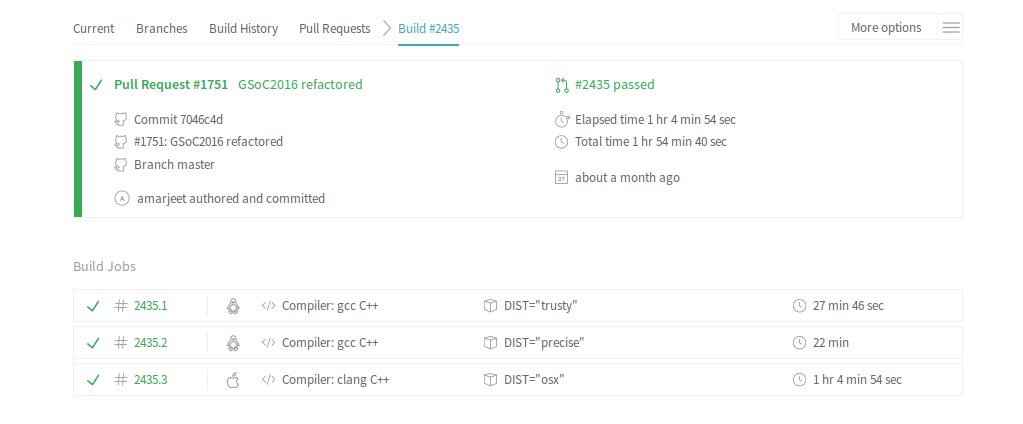
\includegraphics[width=\linewidth]{images/travis}
         \caption{Travis test summary for 3 different OS }
         \label{fig:travis}
     \end{figure}
   
     \item \textbf{Regression Testing:} It is done by running the test cases developed for the OpenSCAD before the New changes are made to check whether new Changes doesn't produce abnormal behavior. \ref{fig:generalTest}
   
     \begin{figure}
         \centering
         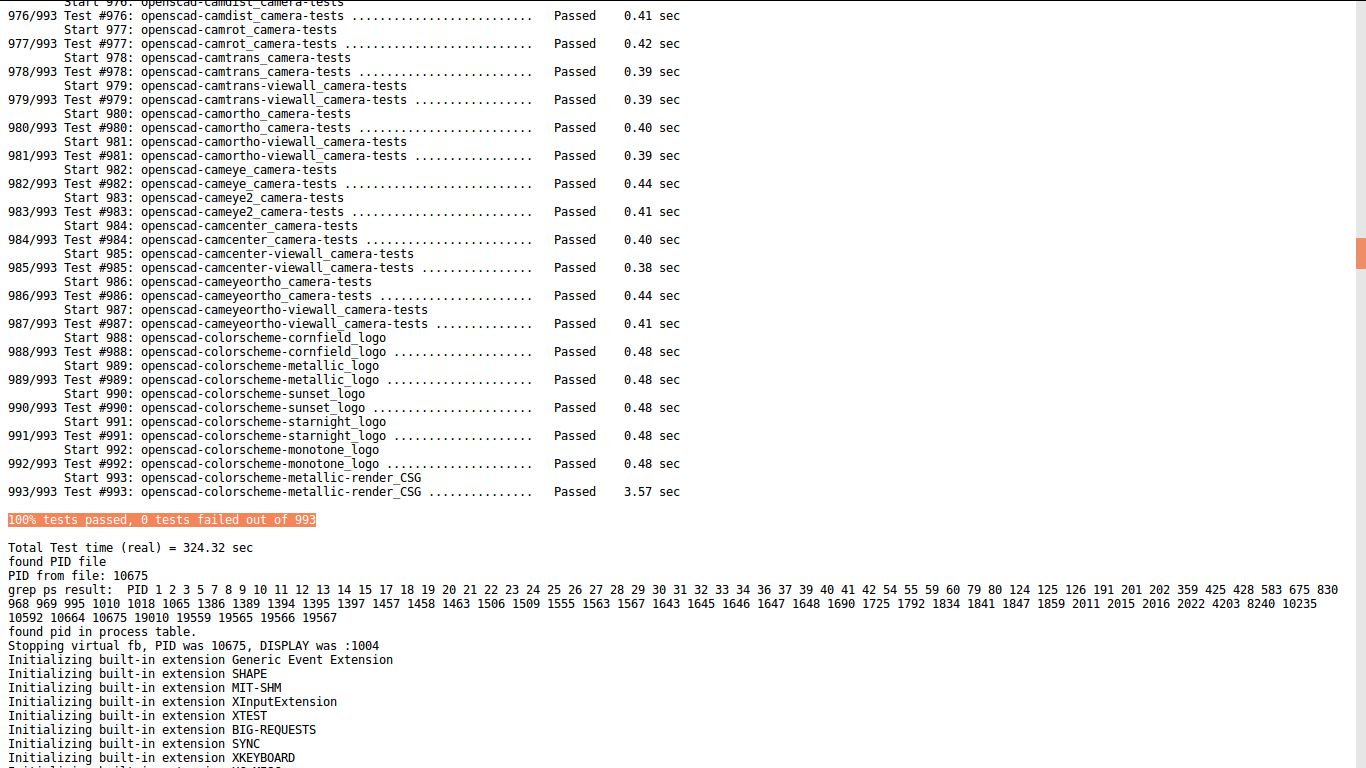
\includegraphics[width=\linewidth]{images/generalTest}
         \caption{Test whole software after Integration}
         \label{fig:generalTest}
     \end{figure}
   
     \item \textbf{Black Box Testing:} In this Testing, the for given set of input and the output is matched with the expected output. \ref{fig:ctest}
   
     \begin{figure}
         \centering
         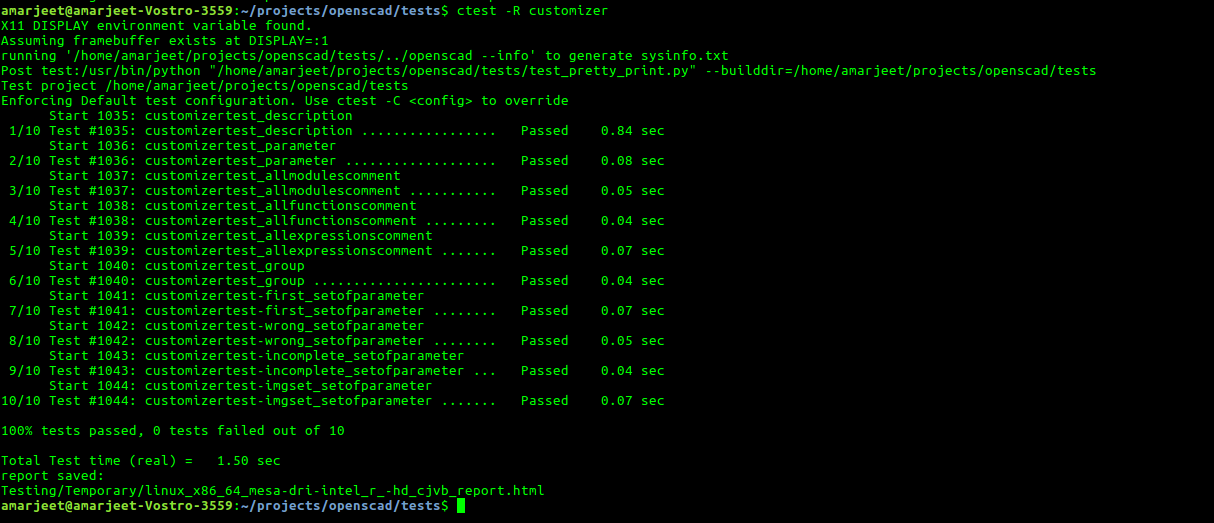
\includegraphics[width=\linewidth]{images/ctest}
         \caption{Tests on ctest}
         \label{fig:ctest}
     \end{figure}
   
 \end{enumerate}

\begin{figure}
    \centering
    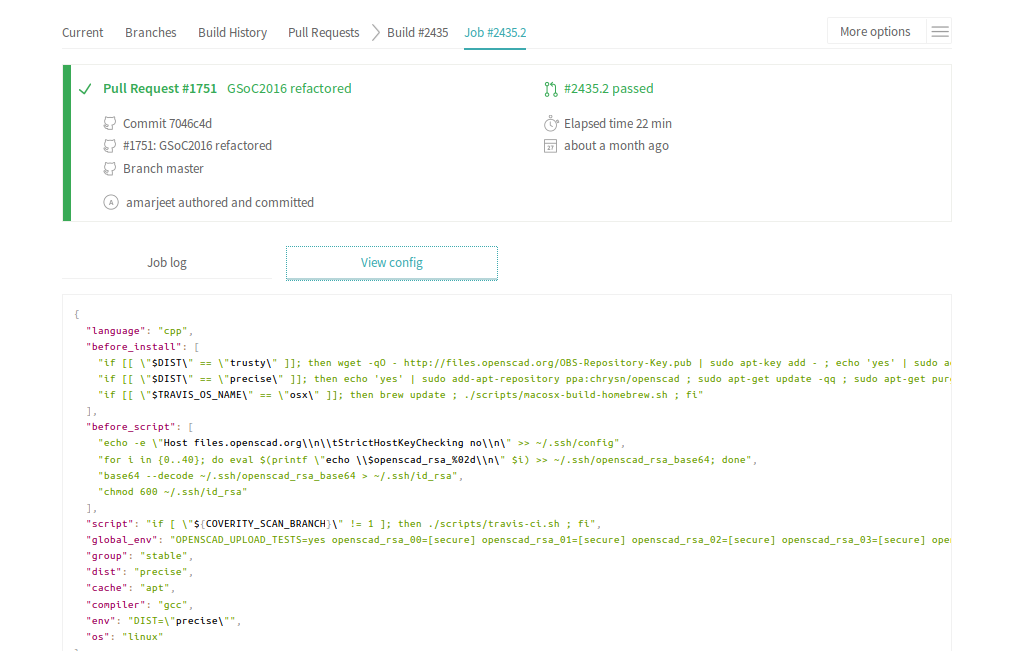
\includegraphics[width=\linewidth]{images/travisSpecific}
    \caption{Configuration and summary of single enviorment}
    \label{fig:travisSpecific}
\end{figure}
 
After passing above Test suit, our project went through system testing, which was of two types:
\begin{figure}
\centering
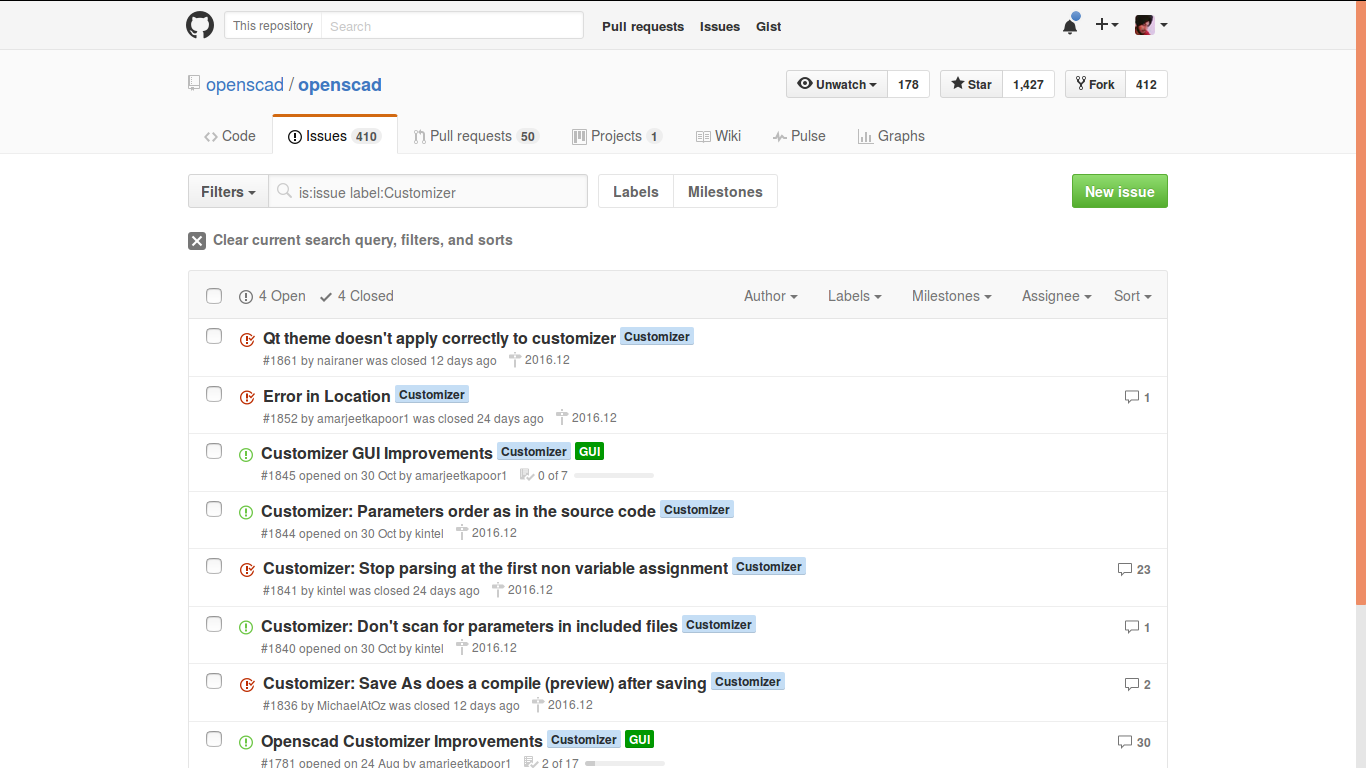
\includegraphics[width=\linewidth]{images/Issues}
\caption{List of Issues provide by Alpha and Beta testers}
\label{fig:Issues}
\end{figure}

\begin{enumerate}
    \item \textbf{Apha Testing}: In this our project was tested my fellow developers working for OpenSCAD community. The issues provided by them were improved and also Testing of User Interface was done. \ref{fig:Issues}
   
    \item \textbf{Beta Testing:} In this our project, was provided to community members and open to all people to test and report the issues or addition that are required to improve User Experience. \ref{fig:Issues}
   
\end{enumerate}

		
		
